\chapter{Implémentation de : Smart Greenhouse } \label{chap:Implémentation de : Smart Greenhouse}
\section{Introduction}
Les chapitres précédent ont expliquées le software  et le hardware  utilisés et comment les deux interagissent. Dans cette partie nous allons présenter diverses technologies et les différentes interfaces de notre application et expliquer l’utilité de chacune d’entre elles. 
\section{Langages de programmation}
\subsection{PHP}
PHP (officiellement, ce sigle est un acronyme récursif pour PHP Hypertext Preprocessor) est un langage de scripts généraliste et Open Source, spécialement conçu pour le développement d'applications web. Il peut être intégré facilement au HTML [18]. 

\begin{figure}[hbt]
\centering
\right
\label{fig:PHP LOGO}

  \fcolorbox{black}{white}{
\includegraphics[width=8cm]{figures/php.jpeg}}
  \caption{PHP logo}
\end{figure}
\newpage
\subsection{C++}
Le C++ est un langage de programmation permettant la programmation sous de multiples paradigmes comme la programmation procédurale, la programmation orientée objet et la programmation générique. C++ est actuellement le 3e langage le plus utilisé au monde. Le langage C++ n'appartient à personne et par conséquent n'importe qui peut l'utiliser sans besoin d'une autorisation ou obligation de payer pour avoir le droit d'utilisation [19].

\begin{figure}[hbt]
\centering
\right
\label{fig:C++ LOGO}

  \fcolorbox{black}{white}{\includegraphics[width=8cm]{figures/c++.jpg}}\caption{C++ logo}
\end{figure}
\newpage
\section{Framework}
\subsection{Laravel}
LARAVEL est un Framework du langage de programmation PHP. Créé par Taylor Otwel, ce framework regroupe les meilleures librairies utiles pour créer un site web. En outre, l’excellent framework laravel intègre aussi bien d’autres fonctionnalités exclusives. C’est notamment le cas de son moteur de template Blade [20].
\begin{figure}[hbt]
\centering
\label{fig:Laravel LOGO}

  \fcolorbox{black}{white}{
\includegraphics[width=8cm]{figures/laravel.jpeg}}\caption{Laravel Logo}
\end{figure}
\newline
\newline
\section{Environment}
\subsection{Arduino IDE}
L’environnement de développement intégré Arduino - ou logiciel Arduino (IDE) contient un éditeur de texte pour écrire du code, une zone de message, une console de texte, une barre d’outils avec des boutons pour les fonctions courantes et une série de menus. Il se connecte au matériel Arduino pour télécharger des programmes et communiquer avec eux [21].

\begin{figure}[hbt]
\centering
\right
\label{fig:Arduino IDE LOGO}
 \fcolorbox{black}{white}{
\includegraphics[width=8cm]{figures/arduino.jpeg}}\caption{Arduino IDE}

\end{figure}
\break
\newline
\subsection{Visual Studio Code}
Visual Studio Code est un éditeur de code extensible développé par Microsoft pour Windows, Linux et macOS3. Le code source de Visual Studio Code provient du projet logiciel libre et open source VS Code de Microsoft publié sous la licence MIT permissive [22].

\begin{figure}[hbt]
\centering
\right
\label{fig:VScode LOGO}

  \fcolorbox{black}{white}{
\includegraphics[width=8cm]{figures/vscode.jpeg}}\caption{VS code logo}
\end{figure}

\subsection{Visual paradigme}
Visual Paradigm Online est un outil de conception de diagrammes en ligne en vue d’une programmation. Il est capable de prendre en charge de nombreux diagrammes commerciaux et techniques comme UML, BPMN, URD, DFD et SysML. Cette plateforme possède une interface graphique simplifiant la manipulation de ses fonctionnalités, et s’adapte à votre manière de travailler [23].

\begin{figure}[hbt]
\centering
\right
\label{fig:Visual paradigme LOGO}

  \fcolorbox{black}{white}{
\includegraphics[width=8cm]{figures/vp.jpg}}\caption{Visual Paradigme logo}
\end{figure}


\subsection{Fritzing}
Fritzing est un logiciel libre de conception de circuit imprimé permettant de concevoir de façon entièrement graphique le circuit et d'en imprimer le typon 
[24].

\begin{figure}[hbt]
\centering
\right
\label{fig: Fritzing LOGO}

  \fcolorbox{black}{white}{
\includegraphics[width=10cm]{figures/fritzing.jpeg}}\caption{Fritzing logo}
\end{figure}

\section{SGBD}
\subsection{MySQL}
MySQL est un Système de Gestion de Base de Données (SGBD) parmi les plus populaires au monde. Il est distribué sous double licence, un licence publique générale GNU et une propriétaire selon l’utilisation qui en est faites. La première version de MySQL est apparue en 1995 et l’outil est régulièrement entretenu. [25]
\begin{figure}[hbt]
\centering
\right
\label{fig: MySQL LOGO}

  \fcolorbox{black}{white}{
\includegraphics[width=12cm]{figures/mysql.jpeg}}\caption{MySQL logo}
\end{figure}

\section{Protocole}
\subsection{API}
L'API est une solution informatique qui permet à des applications de communiquer entre elles et de s'échanger mutuellement des services ou des données [26].

\begin{figure}[hbt]
\centering
\right
\label{fig: API Protocol}

  \fcolorbox{black}{white}{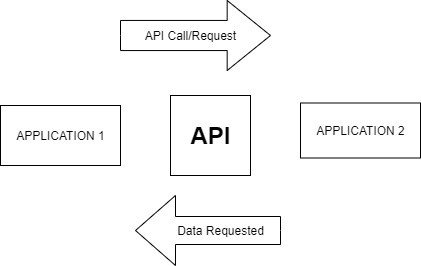
\includegraphics[width=8cm]{figures/api.jpg}}\caption{API Protocol}
\end{figure}

\newpage
\subsection{MVC}
Modèle-vue-contrôleur ou MVC est un motif d'architecture logicielle destiné aux interfaces graphiques, lancé en 1978 et très populaire pour les applications web. Le motif est composé de trois types de modules ayant trois responsabilités différentes : les modèles, les vues et les contrôleurs.

·      Un modèle (Model) contient les données à afficher .

·      Une vue (View) contient la présentation de l'interface graphique .

·      Un contrôleur (Controller) contient la logique concernant les actions effectuées par l'utilisateur.[27]


\begin{figure}[hbt]
\centering
\right
\label{fig: MVC }

  \fcolorbox{black}{white}{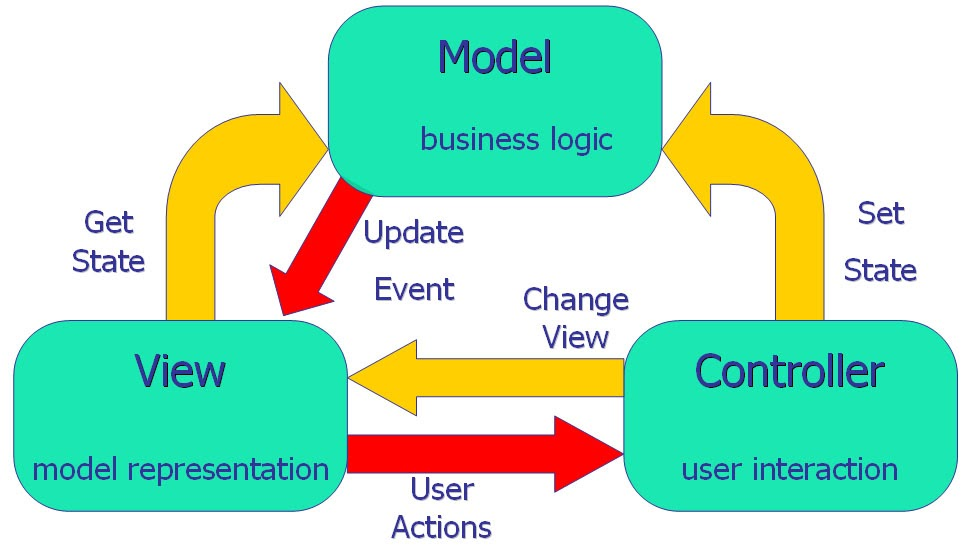
\includegraphics[width=10cm]{figures/MVC.jpeg}}\caption{MVC}
\end{figure}
\section{Application Serveur}
Notre application implémenter sous forme client serveur . Ce serveur communique avec le micro-controlleur a travers l’api mentionner 4.6.1 . Ce meme serveur communique avec l’utilisateur a travers application web mentionner en 4.8. Ce meme serveur tourne sous le serveur d’application PHP . 
\section{Web Application}
L'application permet aux utilisateurs de connaître toutes les évolutions de leurs exploitations, telles que la température de l'exploitation, l'humidité , humidité de  sol et valeur du lumière . Après son implémentation  en PHP nous citons quelque page web du système propose .
\newpage
\section{Réalisation}
Comme indiqué précédemment, notre projet est composée de deux partie á savoir une partie Hardware qui permet de collecter les information nécessaire a une culture saisonnière  et une deuxième software  qui permet de traiter les information collecter du Hardware et de l’utilisateur .
\subsection{Partie Hardware}
Pour répondre au besoin de notre cahier de charge un prototype a été réaliser comme indique sur la figure suivant .

\begin{figure}[hbt]
\centering
\right
\label{fig: Prototype}

  \fcolorbox{black}{white}{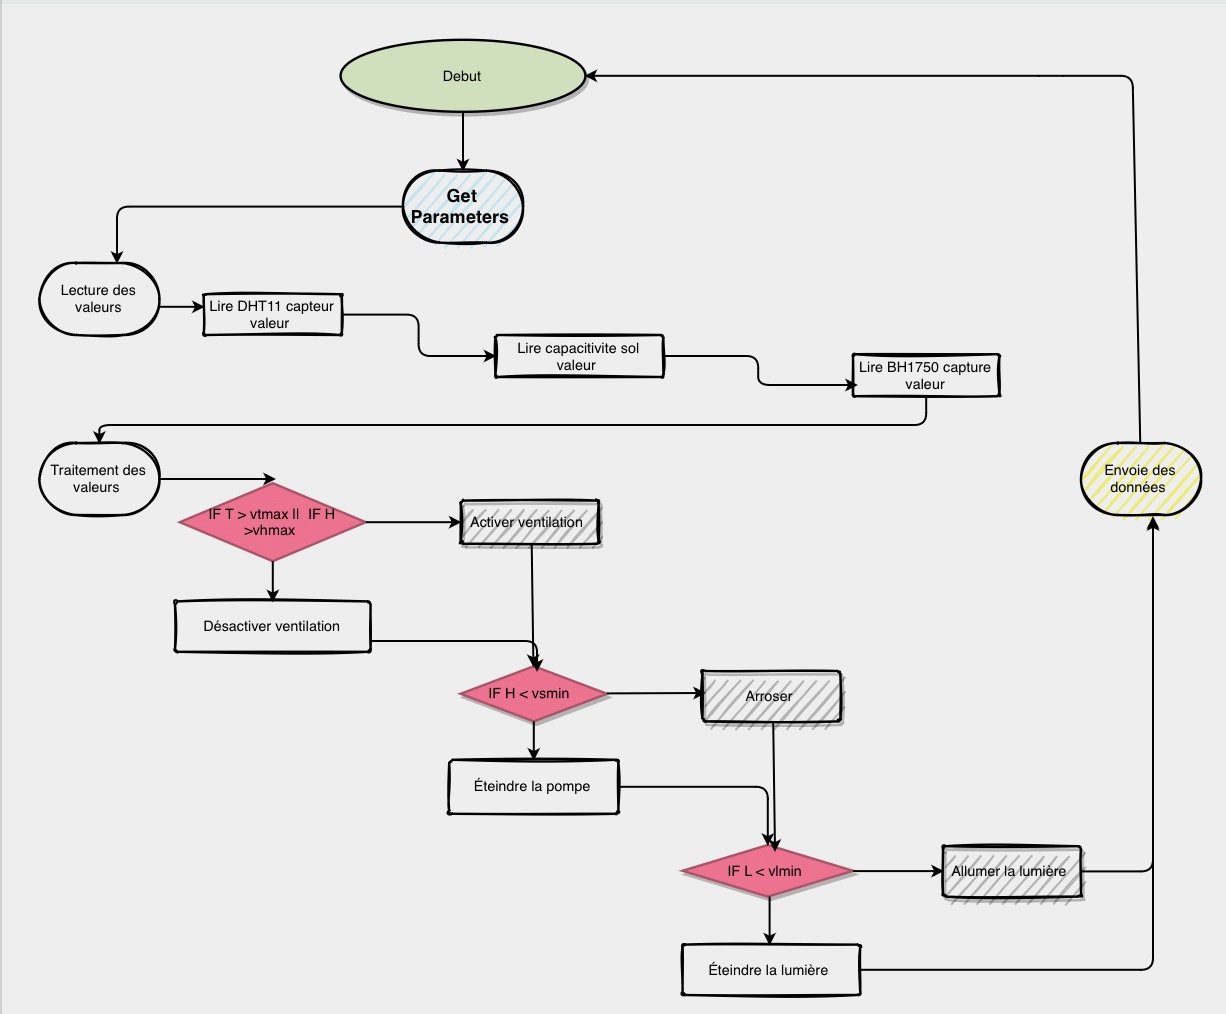
\includegraphics[width=15cm]{figures/agm.jpeg}}\caption{Prototype En cours ...}
\end{figure}

Ce prototype a été réaliser et tester sur un certain nombre de condition 
d’enivrement. Ce test a répondu positivement aux différents exigence. 

%%%%%%%%%%%%%%%%%%%%%%%%%%%%%%%%%%%%%%%%%%%%%%%%%%%%%%%%%%%%%% Software%%%%%%%%%
\break
\newpage
\subsection{Partie Software }
\subsubsection{Utilisation du système}
\textbf{1-  Authentification :}
\newline
Tout utilisateur de notre système doit passer par une authentification comme indiquée par la page web suivant : 



\begin{figure}[hbt]
\centering
\right
\label{fig: Login Page}

  \fcolorbox{black}{white}{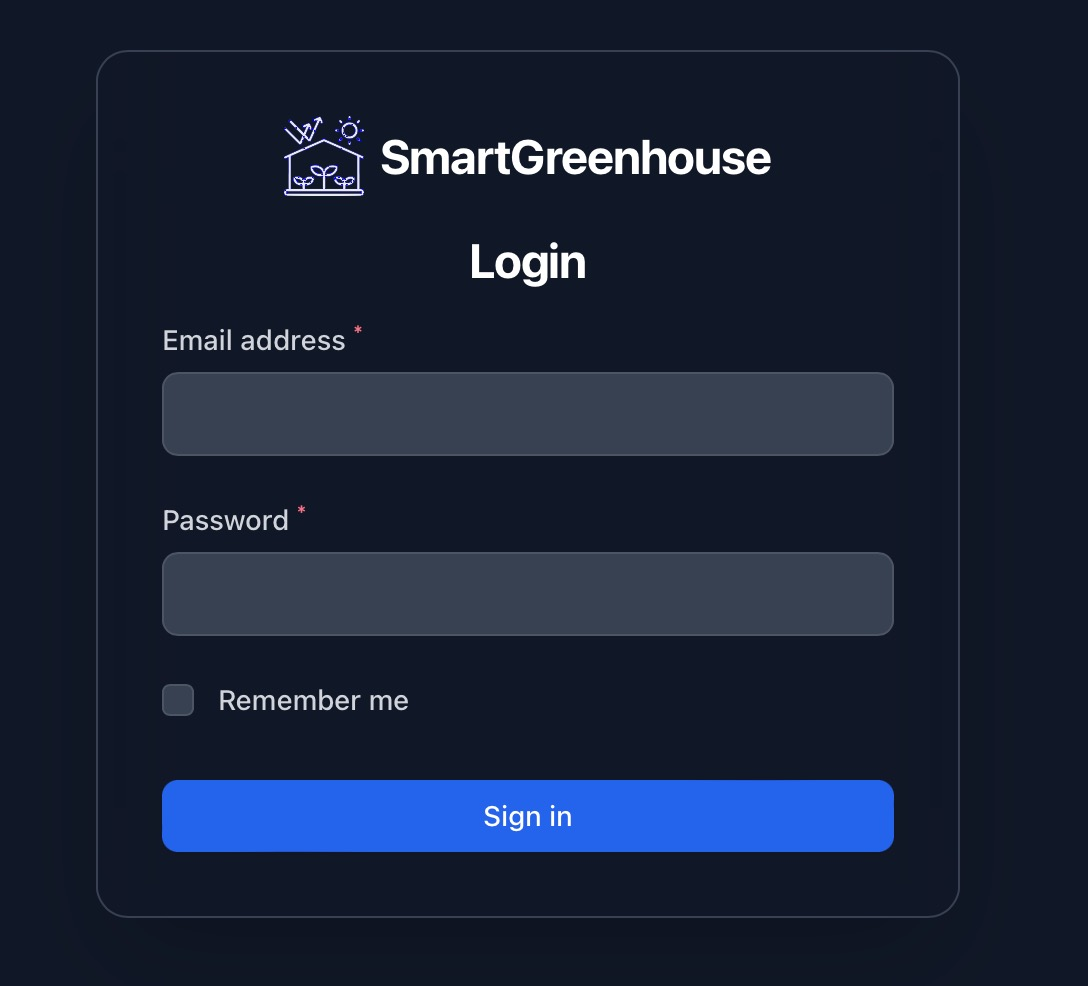
\includegraphics[width=15cm]{figures/Login.jpeg}}\caption{Login Page}
\end{figure}


\textbf{2-  Page d’accueil :}
 Une fois l’utilisateur authentifier, la page d’accueil est afficher (voir figure 4.13). Cette page web illustre   toutes les opérations prévus par ce système. De plus cette page visualise quelque informations standard  sous forme textuelle et graphique .

\begin{figure}[hbt]
\centering
\right
\label{fig: Home Page}

  \fcolorbox{black}{white}{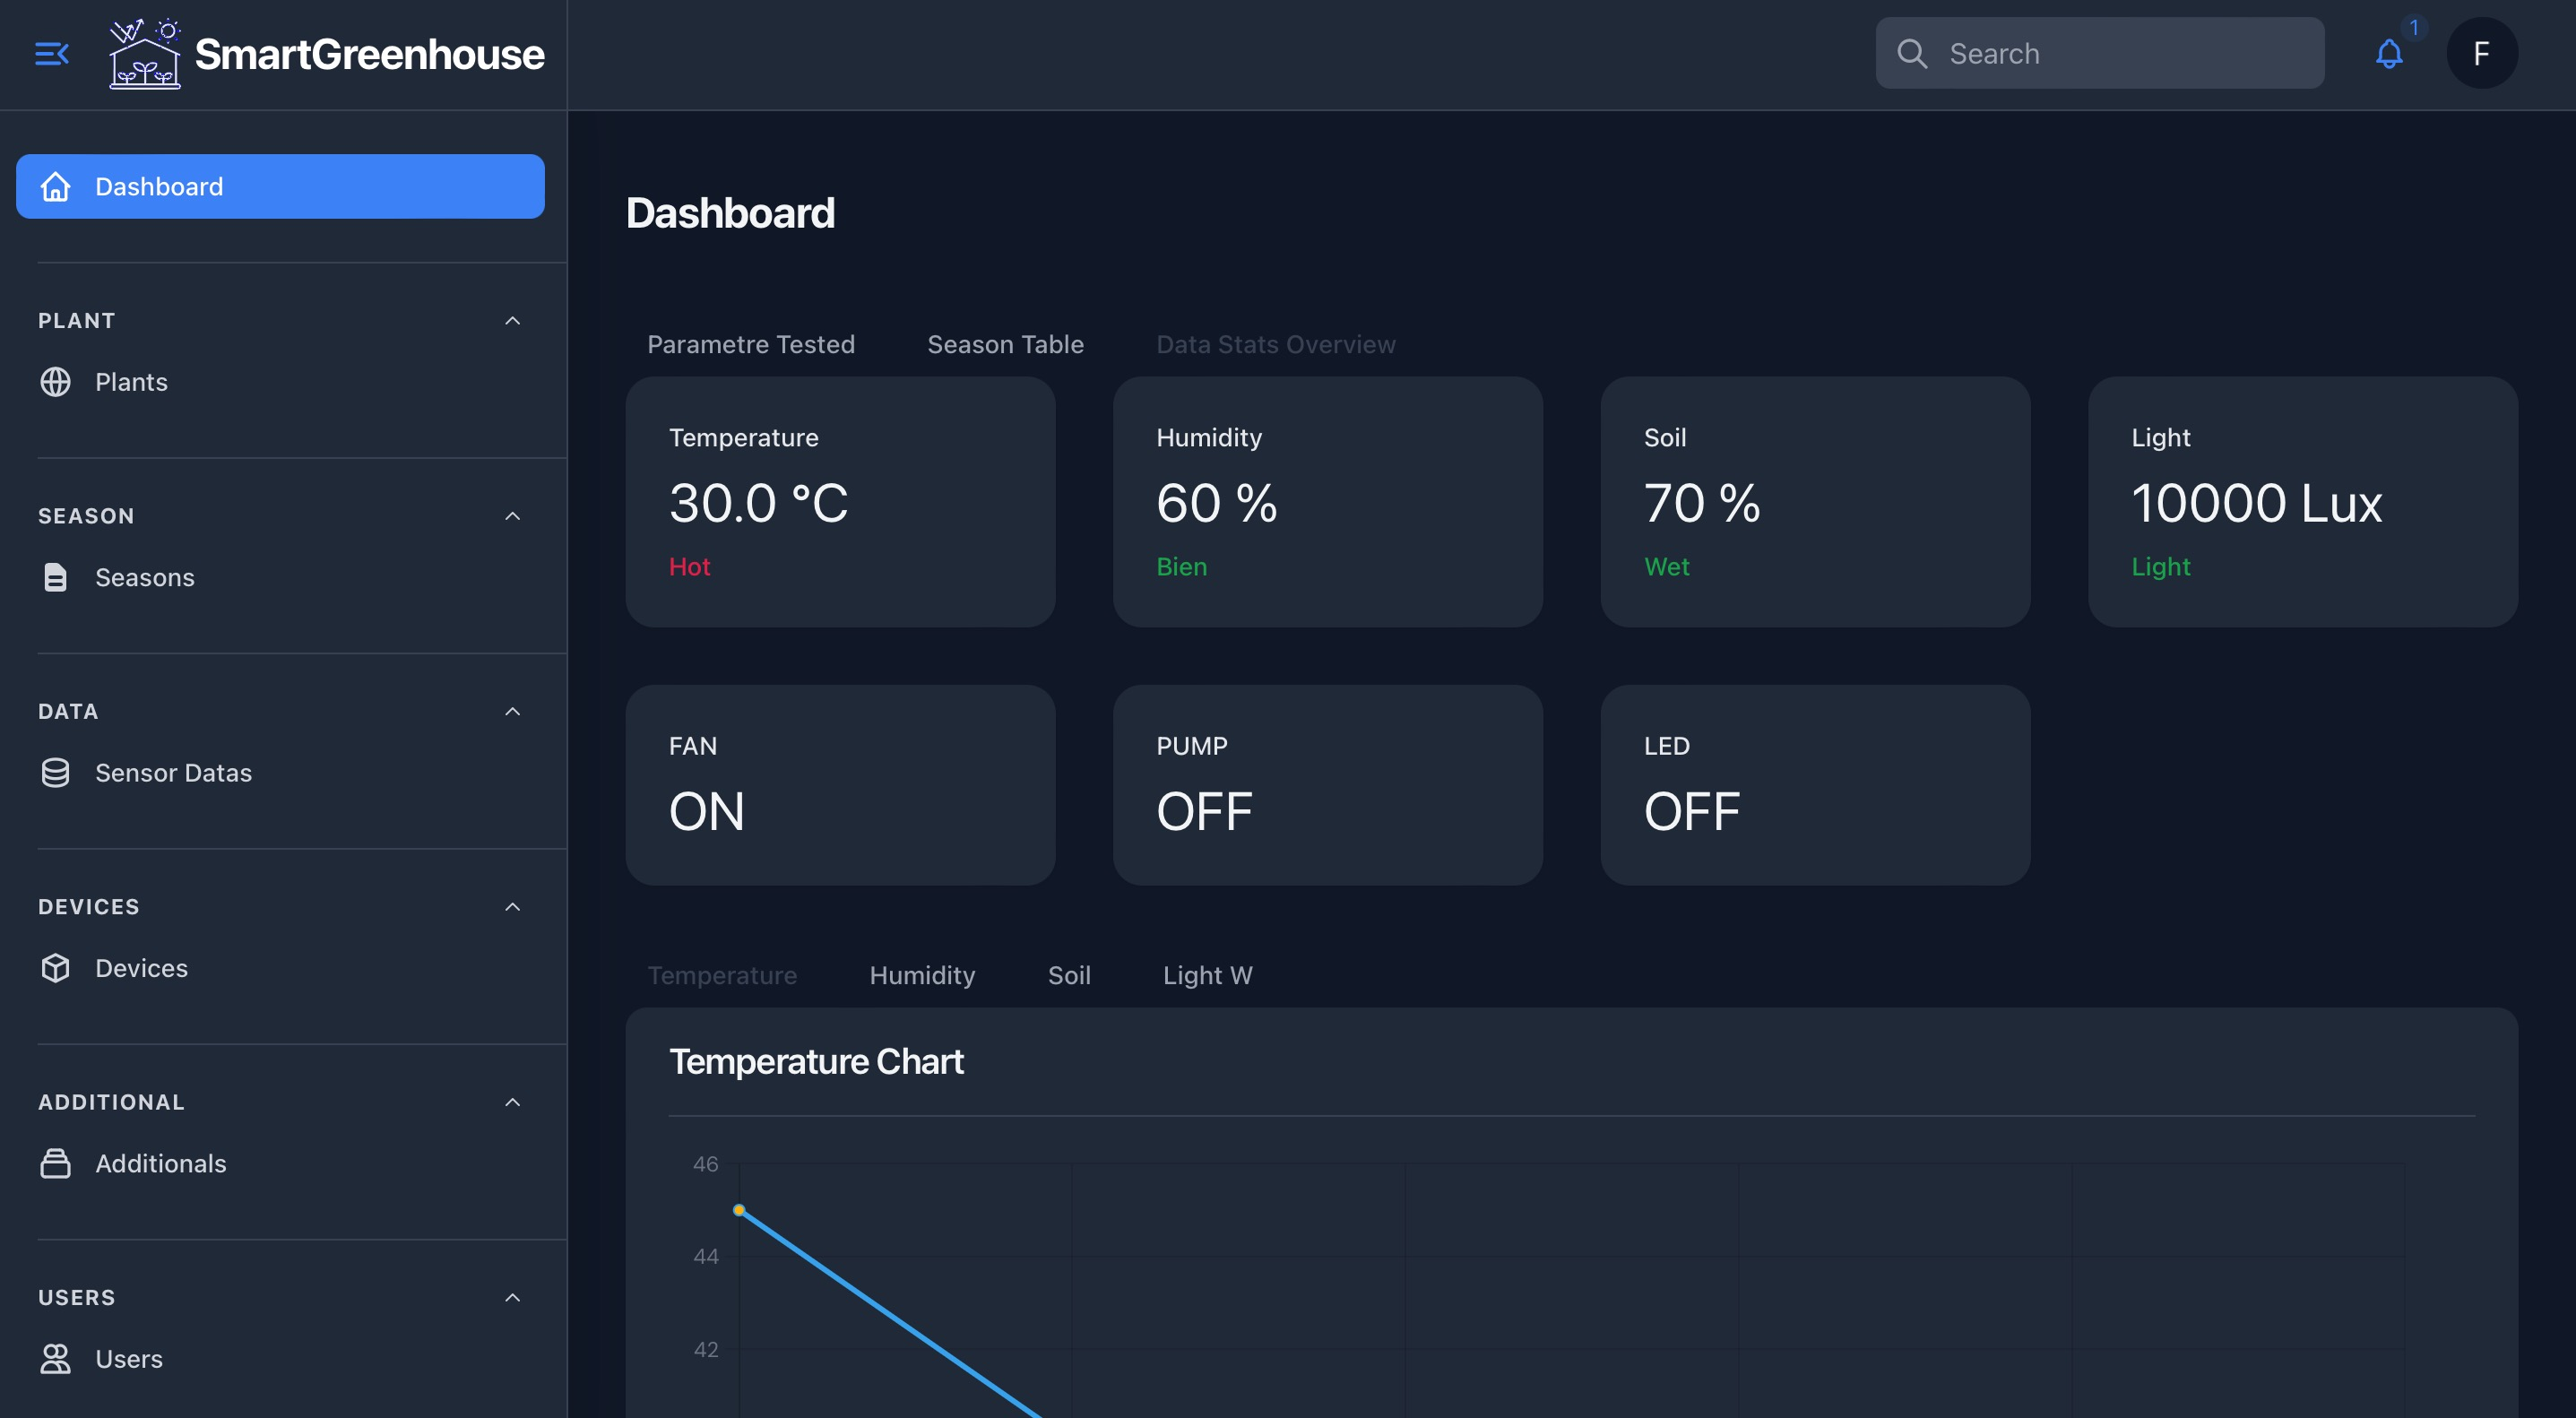
\includegraphics[width=16cm]{figures/HomePage.jpeg}}\caption{Home Page}
\end{figure}
%%%%%%%%%%%%%%%%%%%%%%%%%%%%%%%%% Forms %%%%%%%%%%%%%%%%%%%%%%%%%%%%%%%%%%%%%%
\newpage
\subsubsection{Introduction du données }
\textbf{1-  Formulaire de création d’une nouvelle saison du culture :}
\newline
A chaque nouvelle saison, l’utilisateur doit initier cette dernière on introduisent \newline les données nécessaire comme indiquer sur la figure suivant :

\begin{figure}[hbt]
\centering
\right
\label{fig:Create New Season}

  \fcolorbox{black}{white}{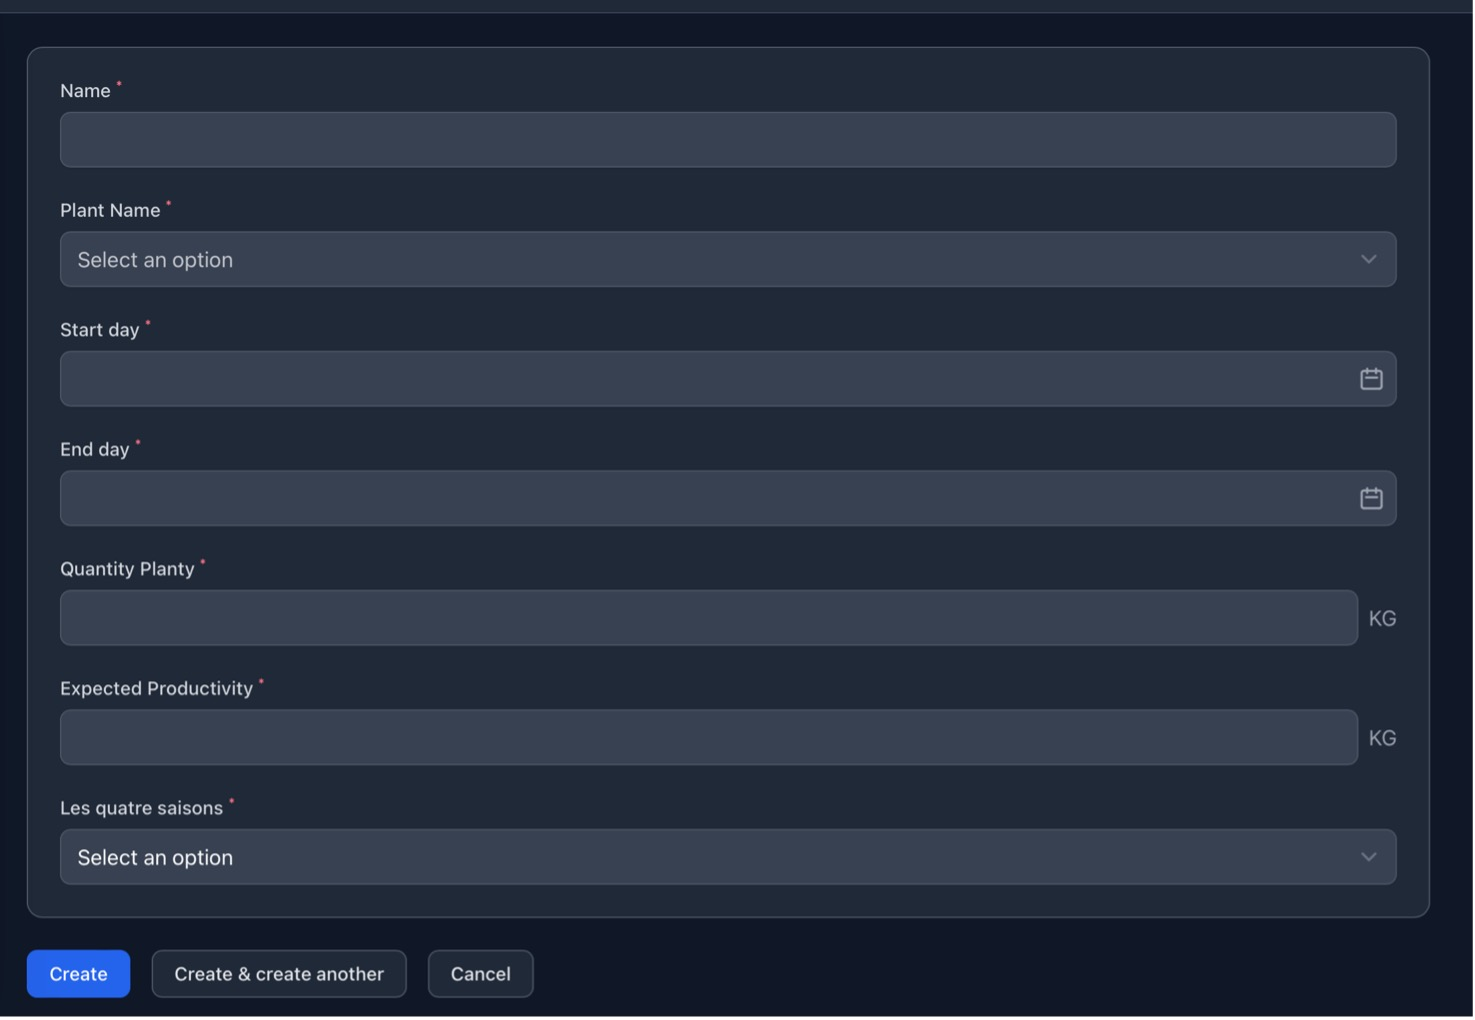
\includegraphics[width=13cm]{figures/formseason.jpg}}\caption{Create New Season}
\end{figure}


\newpage
\textbf{2-  Réglage des paramètres :}
\newline
L’utilisateur peut également modifie les paramétrage de la saison a tout instant en utilisant le page web suivant  .

\begin{figure}[hbt]
\centering
\right
\label{fig:Edit Parametre}

  \fcolorbox{black}{white}{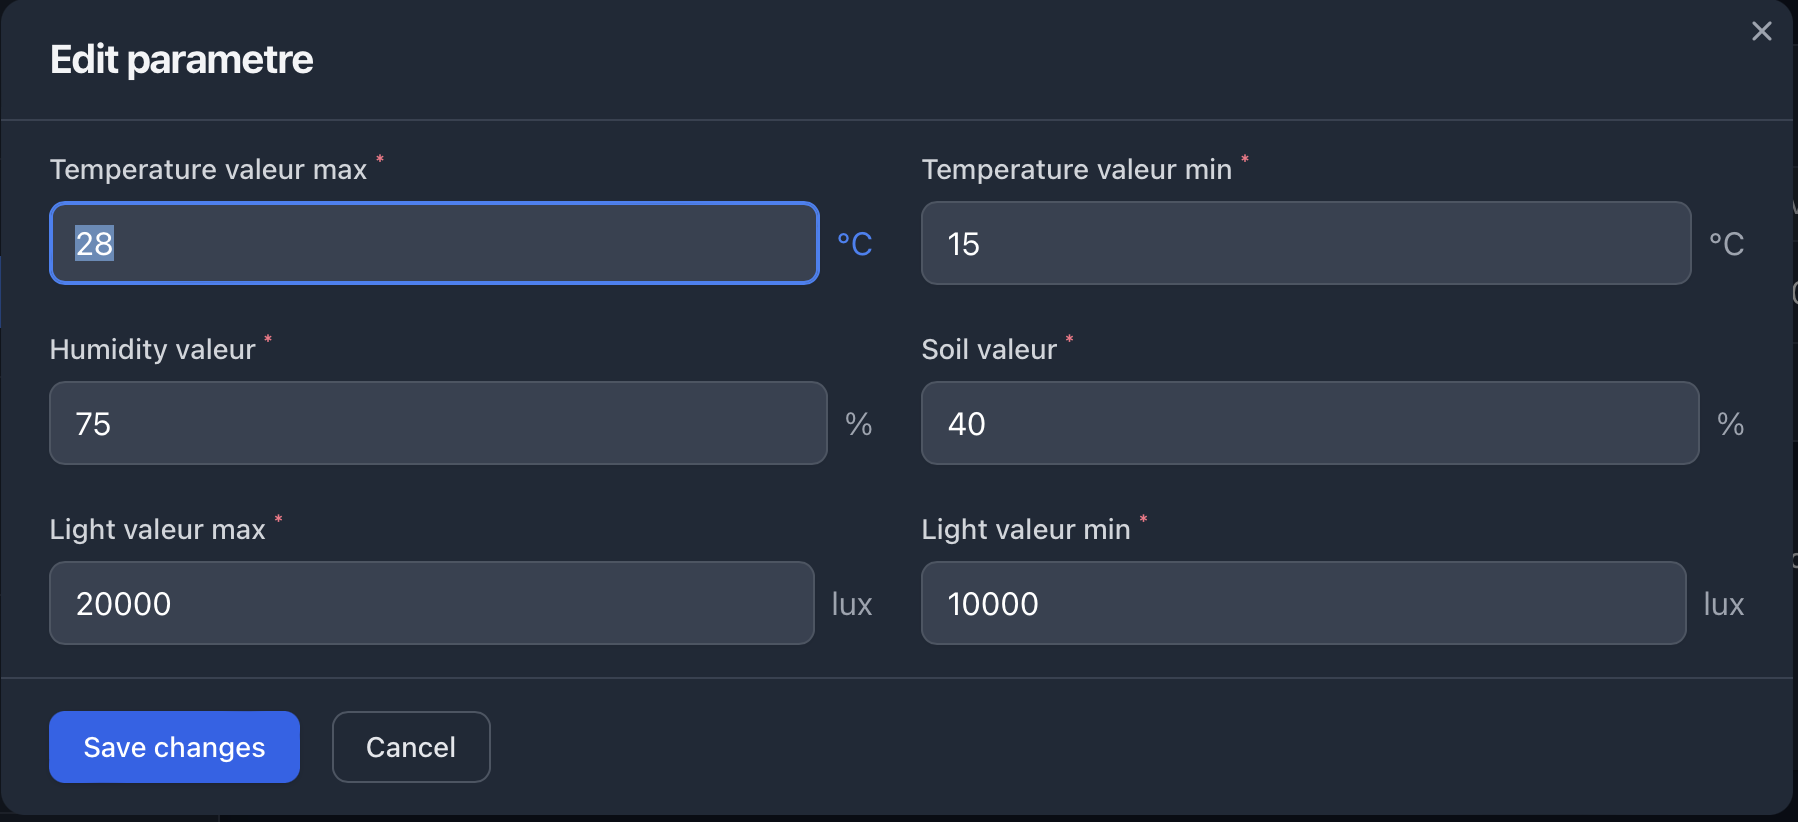
\includegraphics[width=16cm]{figures/parform.png}}\caption{Edit Parametre}
\end{figure}

%%%%%%%%%%%%%%%%%%%%%%%%% Notification %%%%%%%%%%%%%%%%%%%%%%%%%%%%%%%%%%%%
\subsubsection{Notification}
Utilisateur est  notifier pour toute anomalies du hardware.
\begin{figure}[hbt]
\centering
\right
\label{fig:Notification}

  \fcolorbox{black}{white}{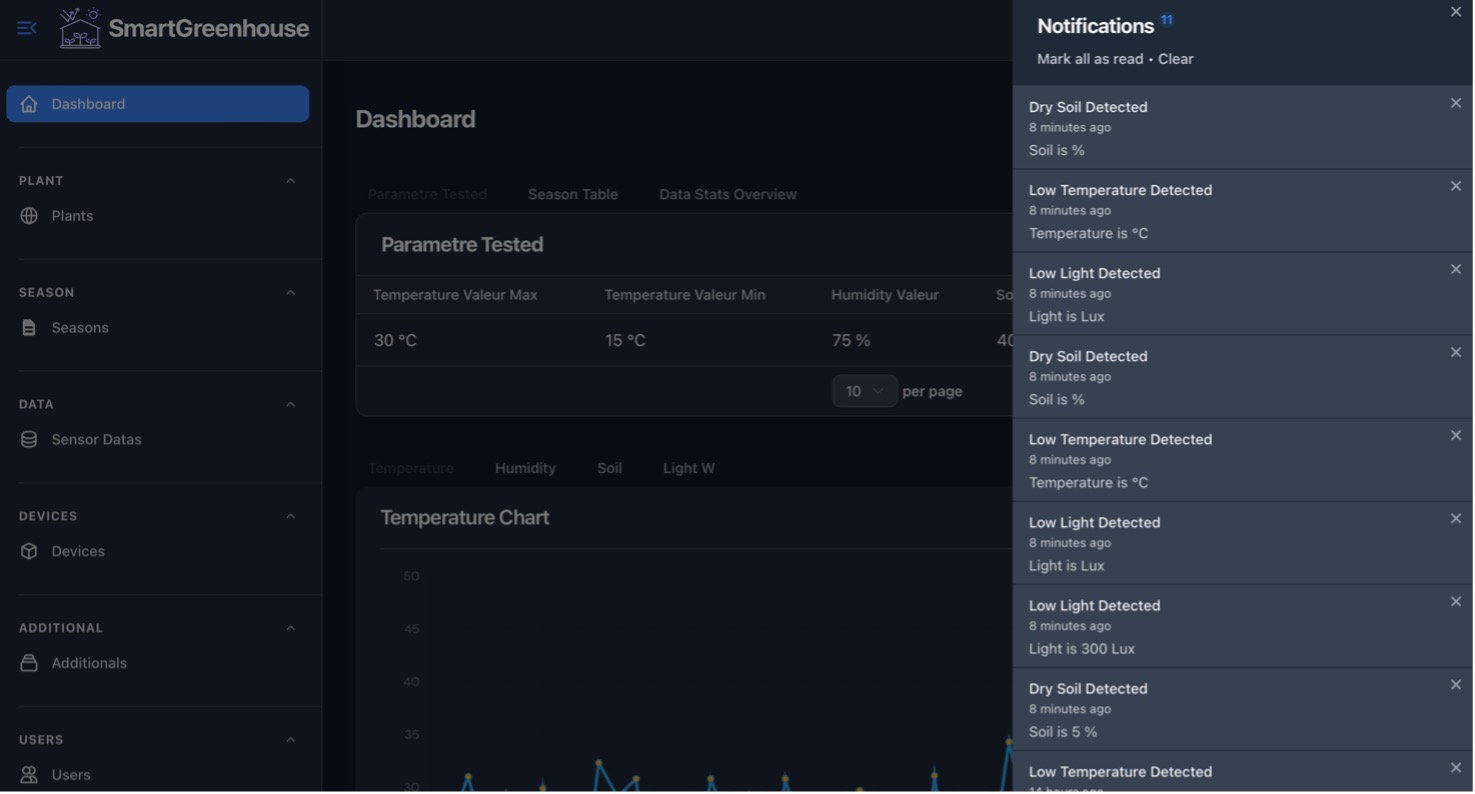
\includegraphics[width=15.5cm]{figures/notification.jpeg}}\caption{Notification Center}
\end{figure}

% Dashboards %%%%%%%%%%%%%%%%%%%%%%%%%%%%%%%%%%%%%%%%%%%%%%%%%%%%%%%%%%%%%%%%%
\newpage
\subsubsection{Dashboards}
Le menu de page d’accueil offre un certain nombre de dashboard dont voici quelque 

\textbf{1-  Dashboard des évènements de données}

\begin{figure}[hbt]
\centering
\right
\label{fig: SensorData Dashboard}

  \fcolorbox{black}{white}{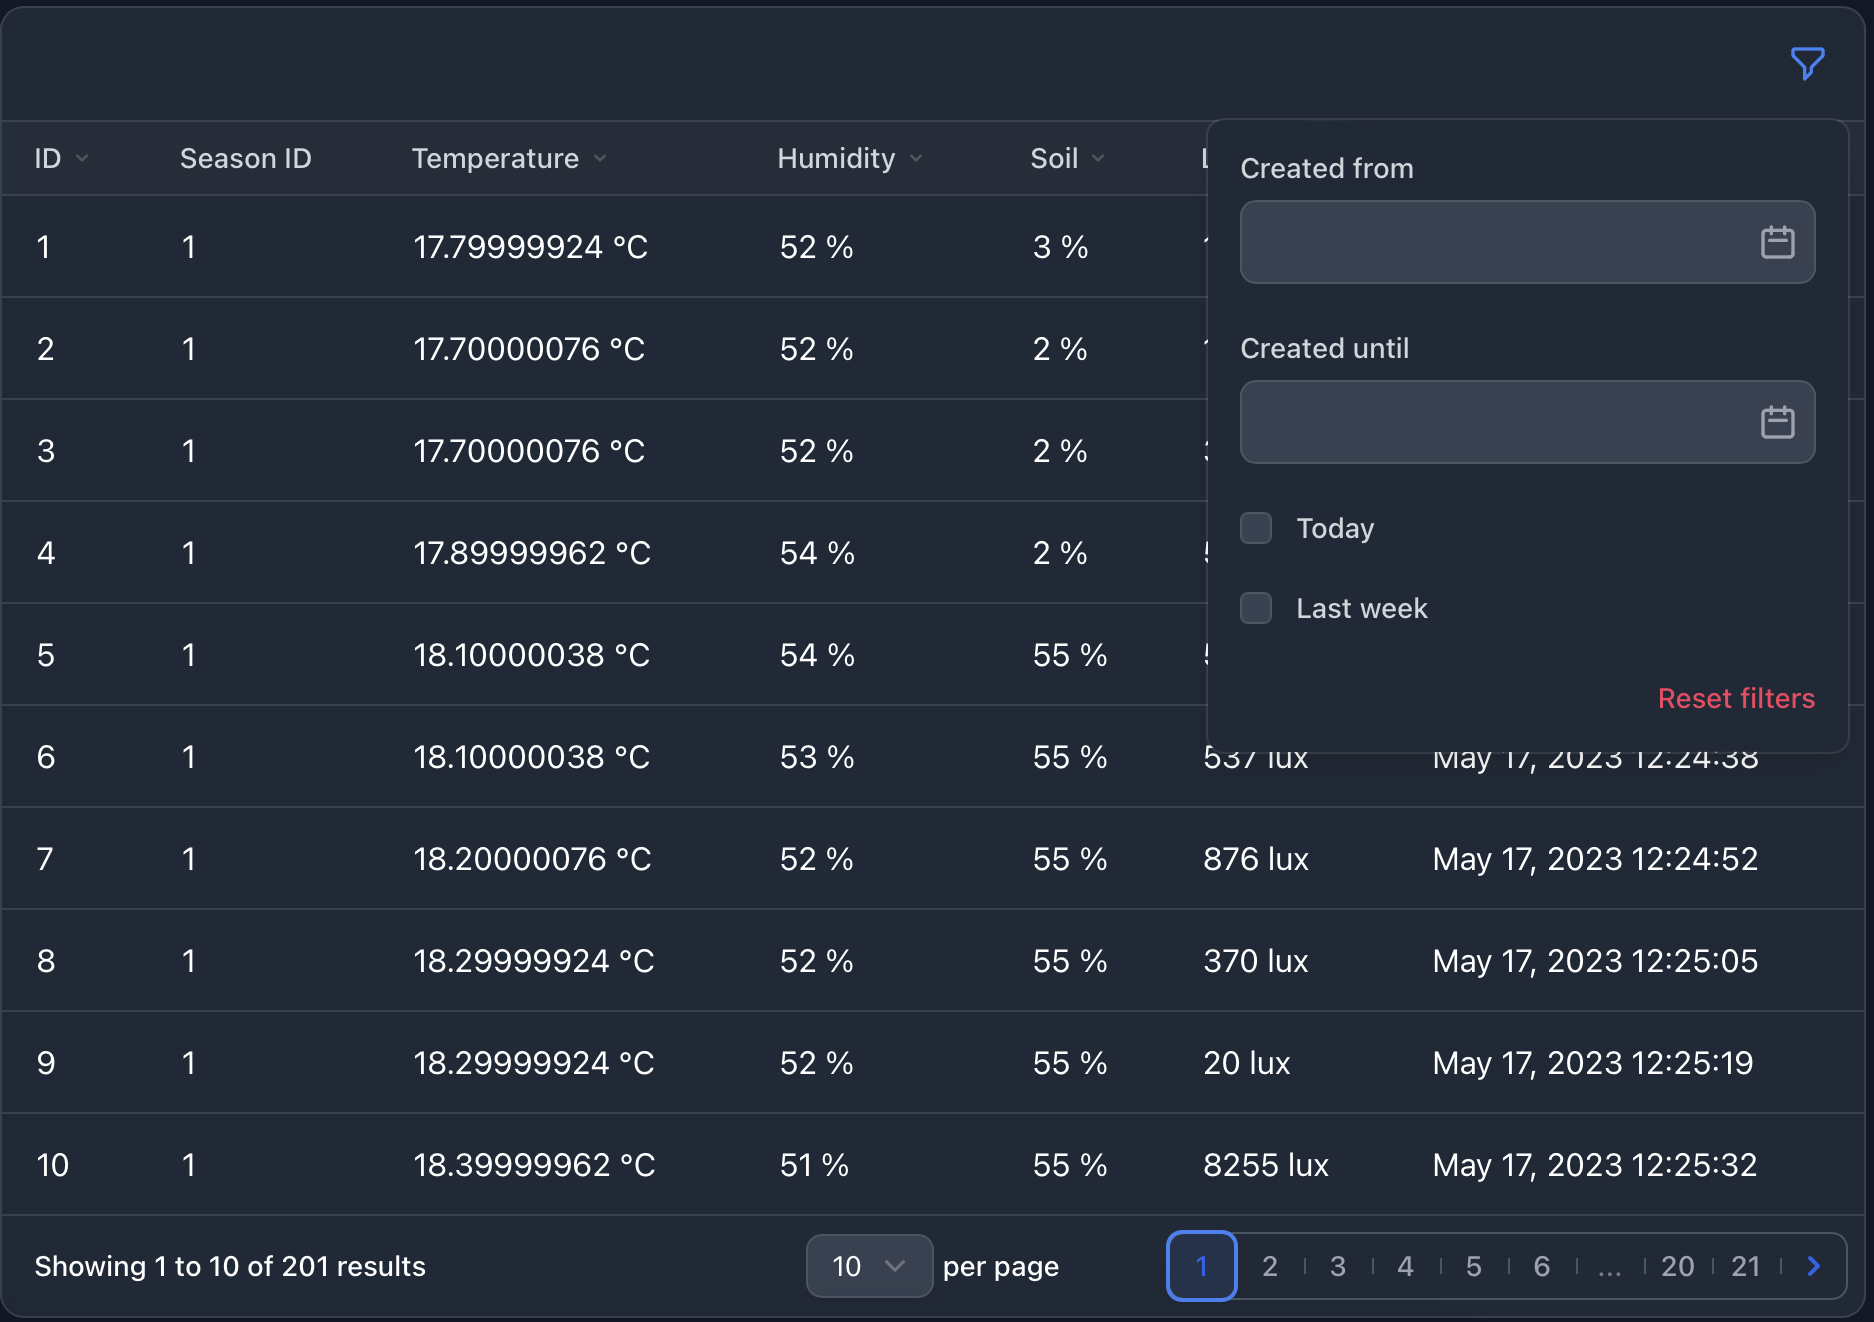
\includegraphics[width=18cm]{figures/de.png}}\caption{SensorData Dashboard}
\end{figure}

Ce Dashboard visualise les évènements qui on eux lieu durant une période . 
\break
\newline
\textbf{2-  Dashboard Graphe linière}
\newline
Ce Dashboard affiche des courbes graphiques montrant les valeurs de température, d’humidité , humidité de  sol et valeur du lumière durant la saison.
\begin{figure}[hbt]
\centering
\right
\label{fig: Graphe Linear de Temperature}

  \fcolorbox{black}{white}{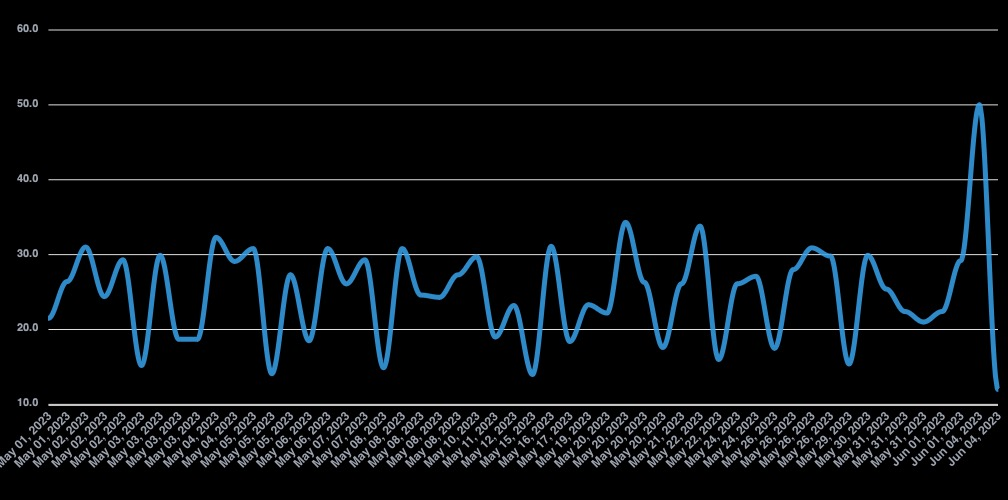
\includegraphics[width=16cm]{figures/Tempurature.jpeg}}\caption{Graphe Linear de Temperature}
\end{figure}

\newpage
il peut filtrer par date :

\begin{figure}[hbt]
\centering
\right
\label{fig: Graphe Linear de Temperature Filtré}

  \fcolorbox{black}{white}{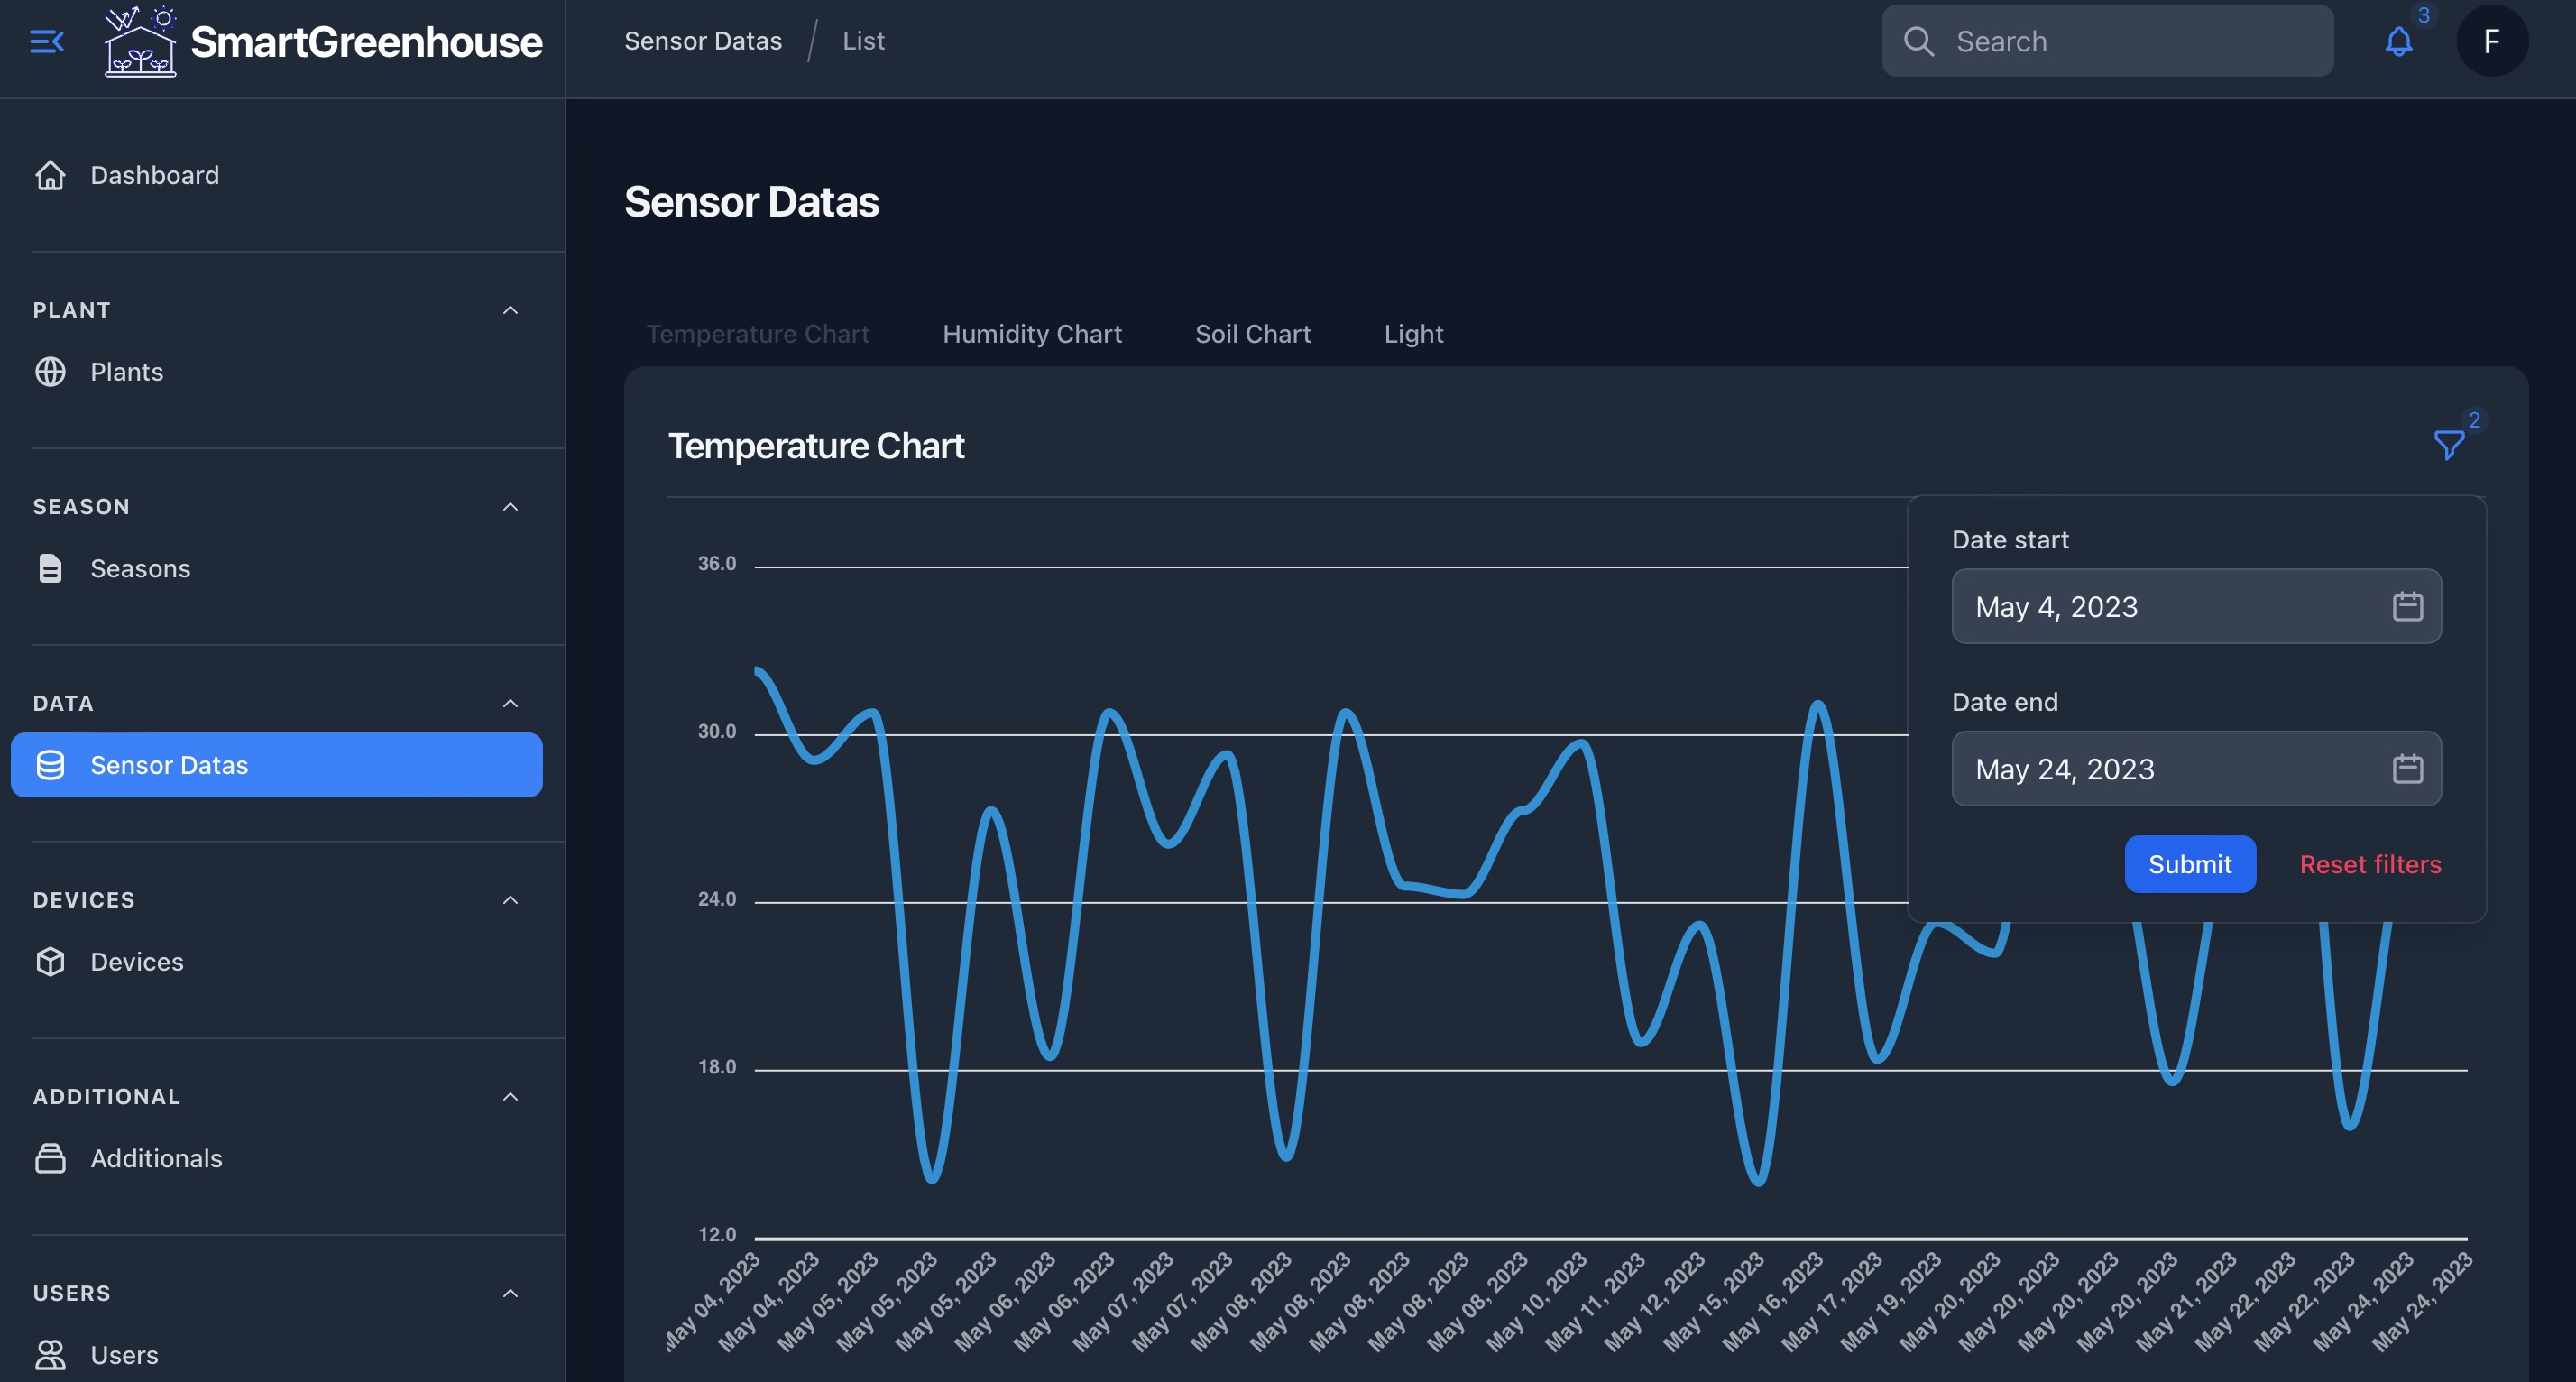
\includegraphics[width=18cm]{figures/Filtrage.jpeg}}\caption{Graphe Linear de Temperature Filtré}
\end{figure}

\newpage

\textbf{3-  Dashboard des états tous dispositifs}
\newline
Un Dashboard de visualisation des statuts de tous les dispositifs disponible dans le système hardware .
\begin{figure}[hbt]
\centering
\right
\label{fig: Devices Data }

  \fcolorbox{black}{white}{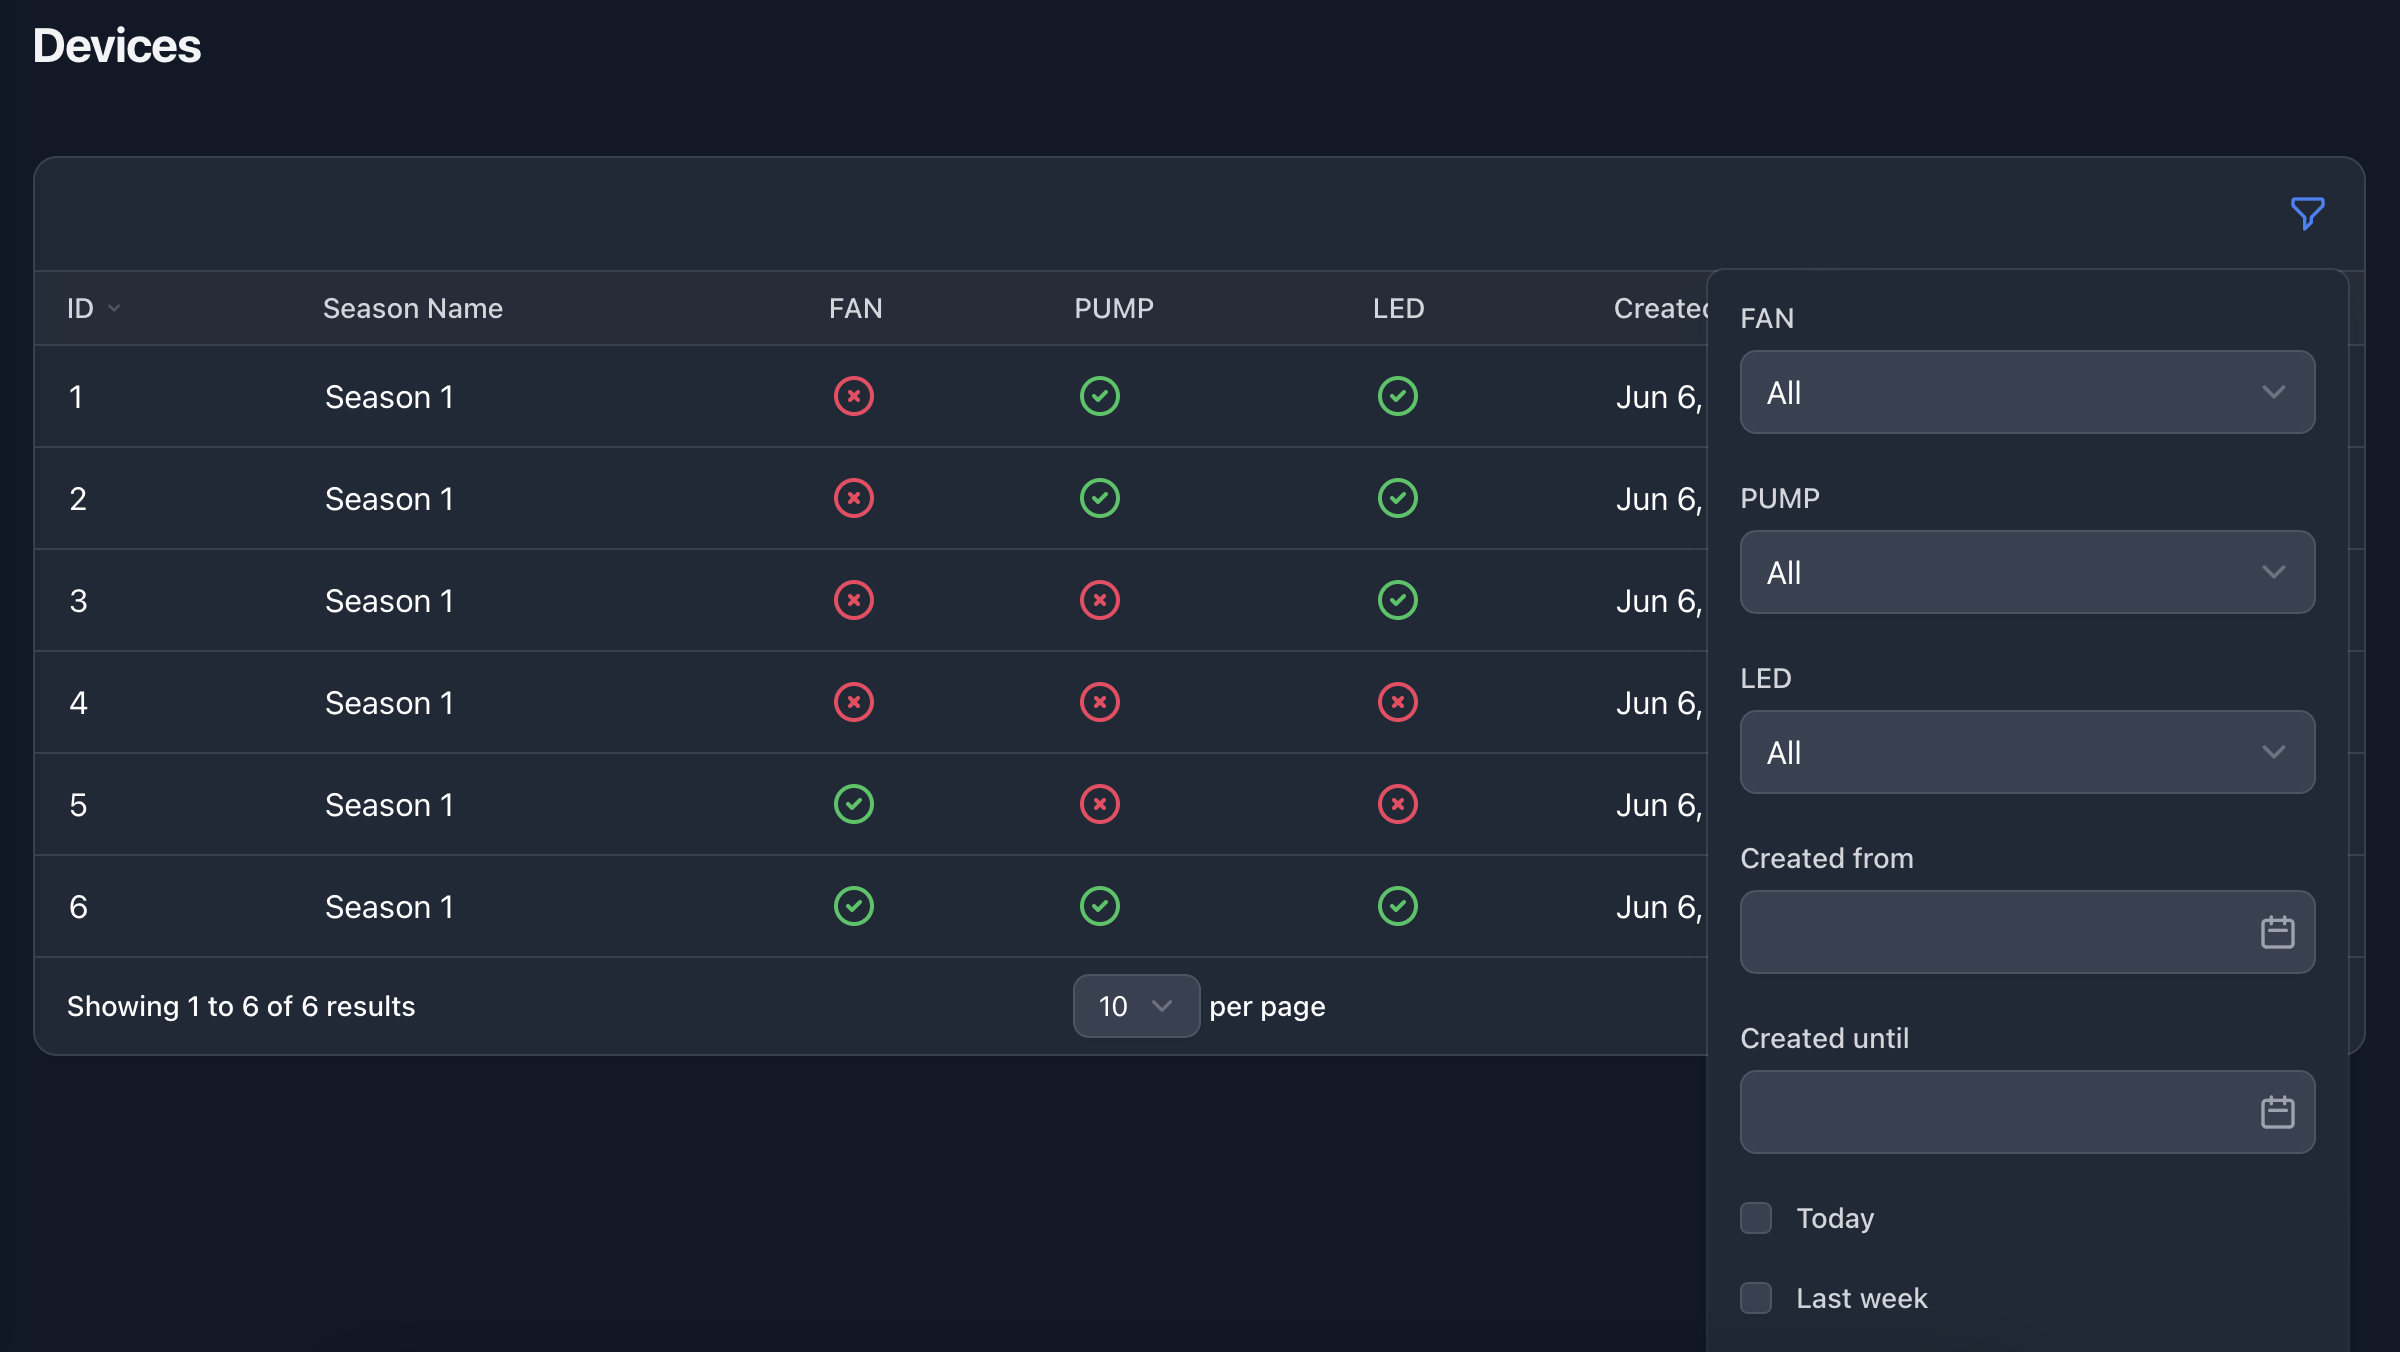
\includegraphics[width=18cm]{figures/edaaa.png}}\caption{Devices Data}
\end{figure}

\textbf{4-  Dashboard Saison Vue}
\newline
Dans ce Dashboard en présente  les informations de saison choisi ansi que tout \newline les relations lie a cette saison comme paramètre, évènement de données, évènements de dispositifs, additionnels et observation.

\begin{figure}[hbt]
\centering
\right
\label{fig:Season View}

  \fcolorbox{black}{white}{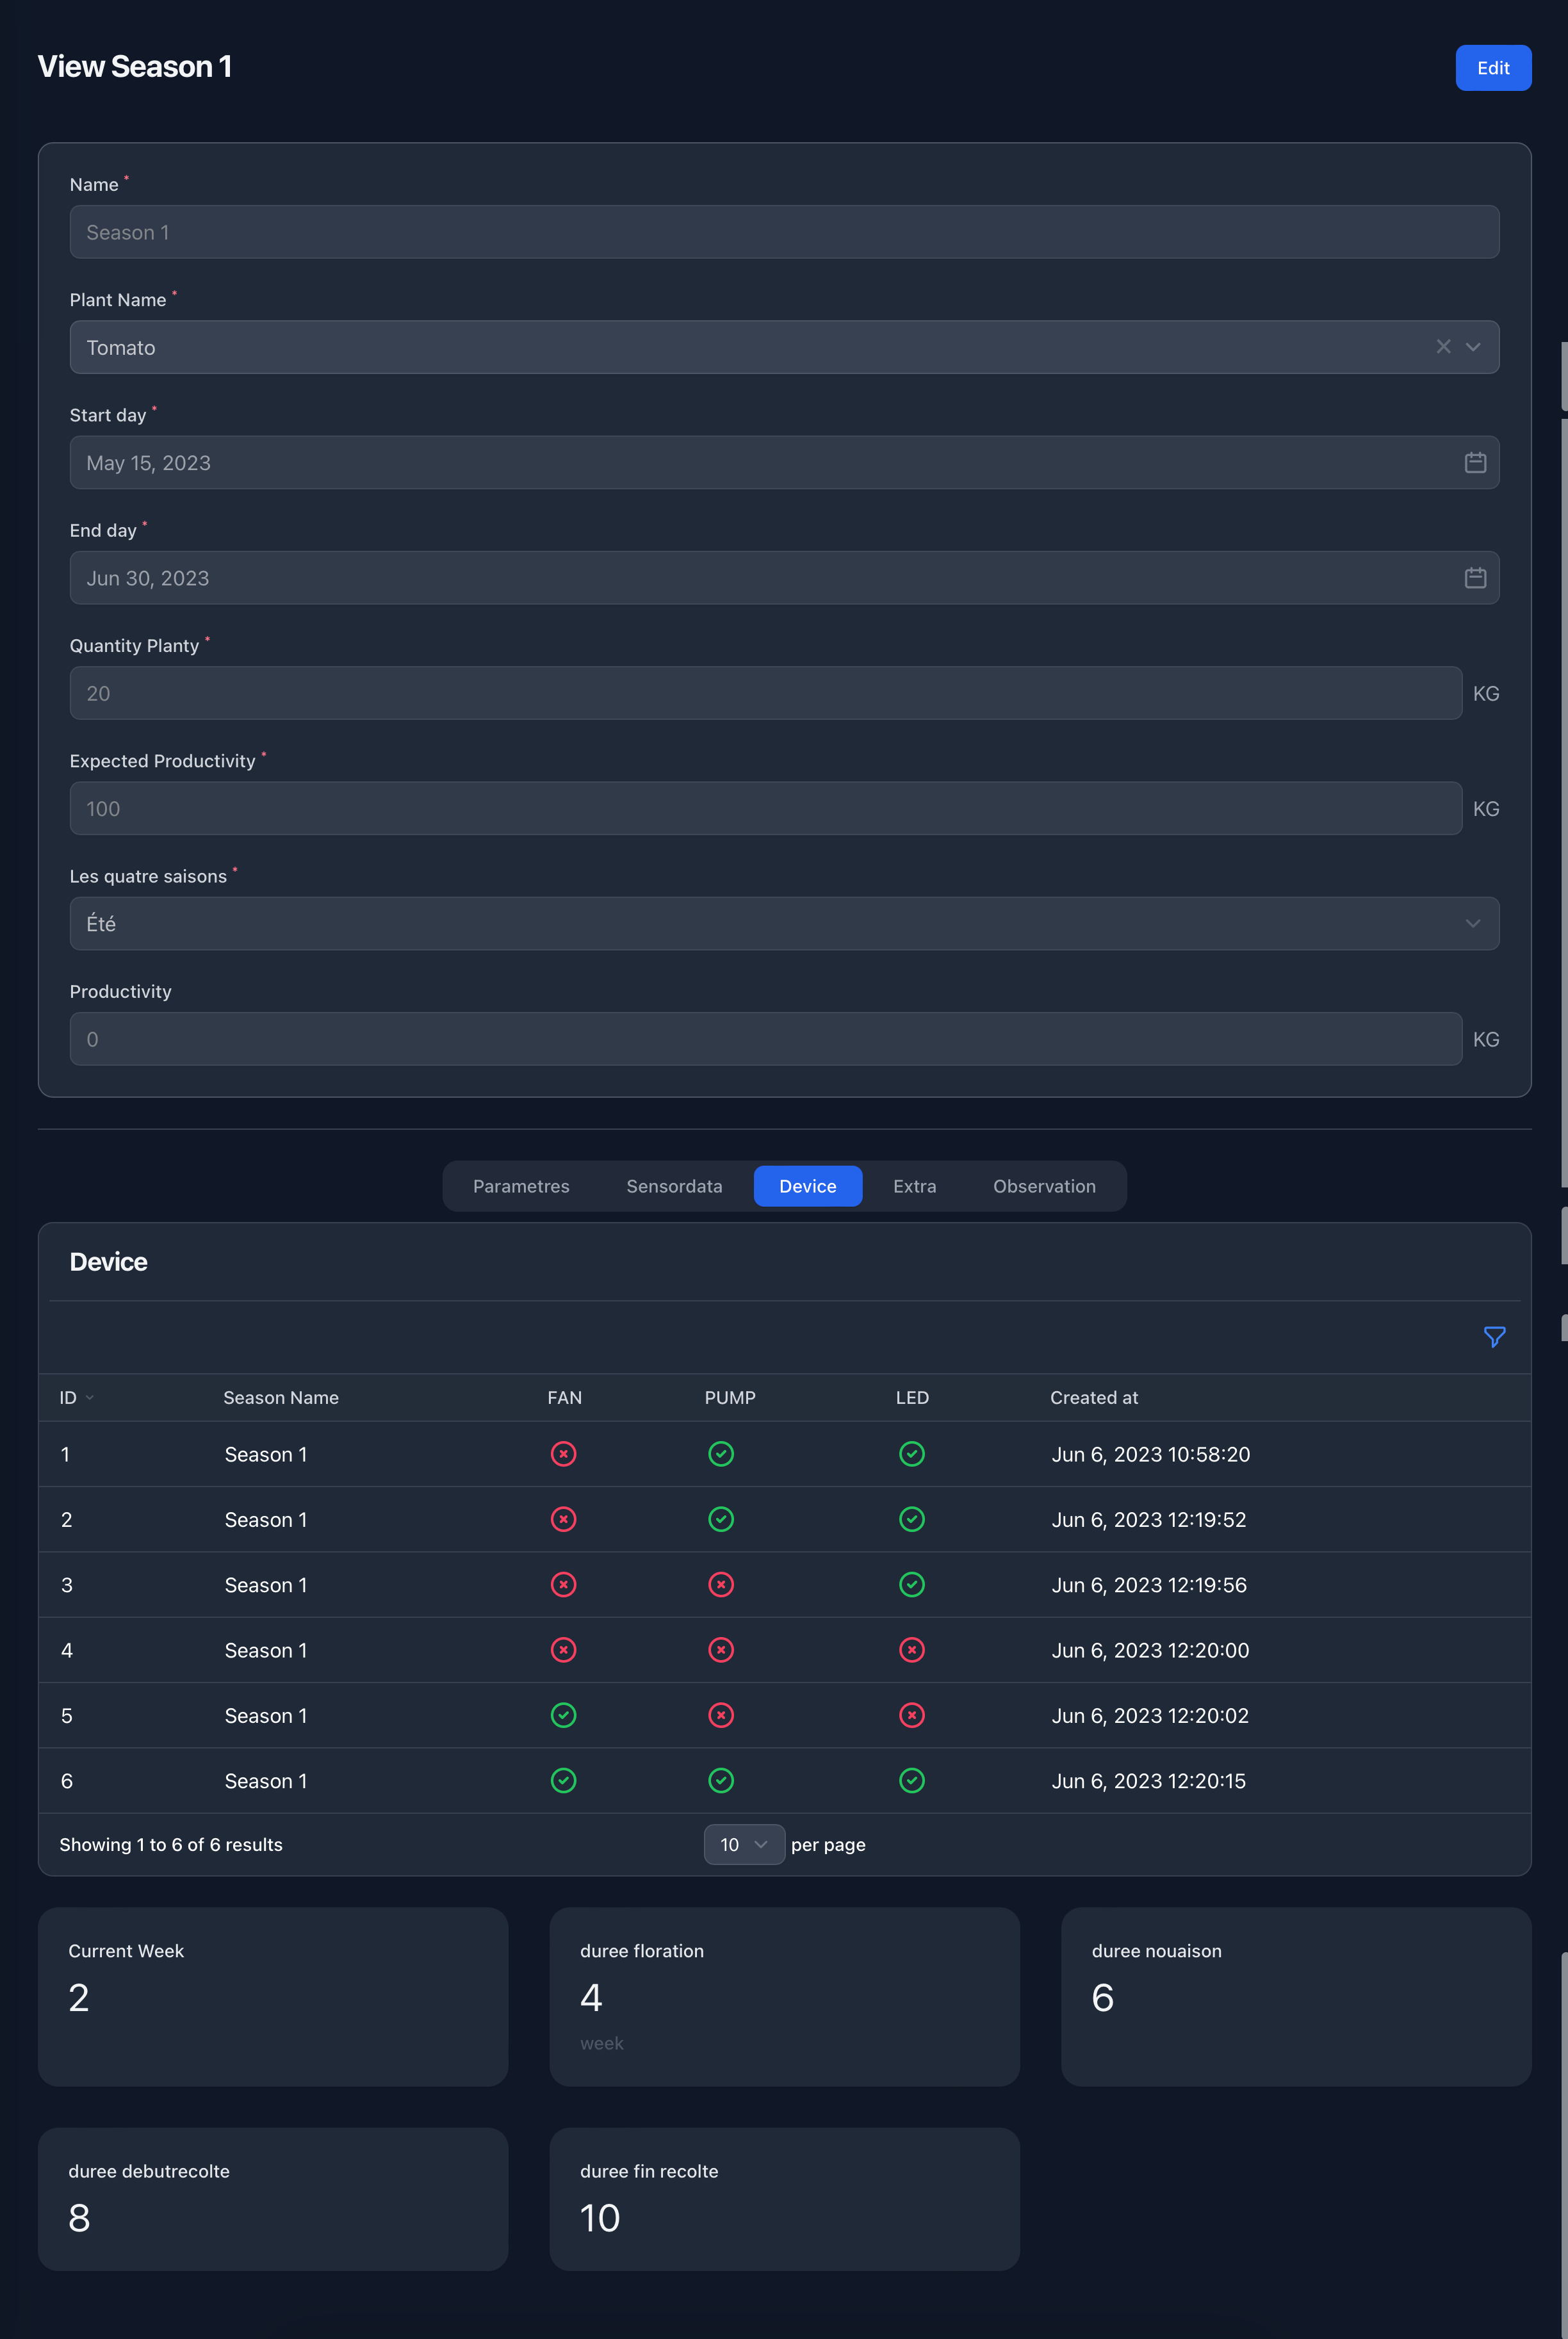
\includegraphics[width=13cm]{figures/SeasonView.png}}\caption{Season View}
\end{figure}
\newpage
\section{Conclusion}

En utilisons les outils et les langages indique dans ce chapitre, un prototype (Hardware et Software)  a été réalisé et tester sous diffèrent condition environnementale et a donné satisfaction. 
